\begin{anexosenv}

\partanexos
    
\chapter{Primeiro Anexo}

\begin{figure}[H]
    \centering
    \caption{Online Judge - Browse Problems}
    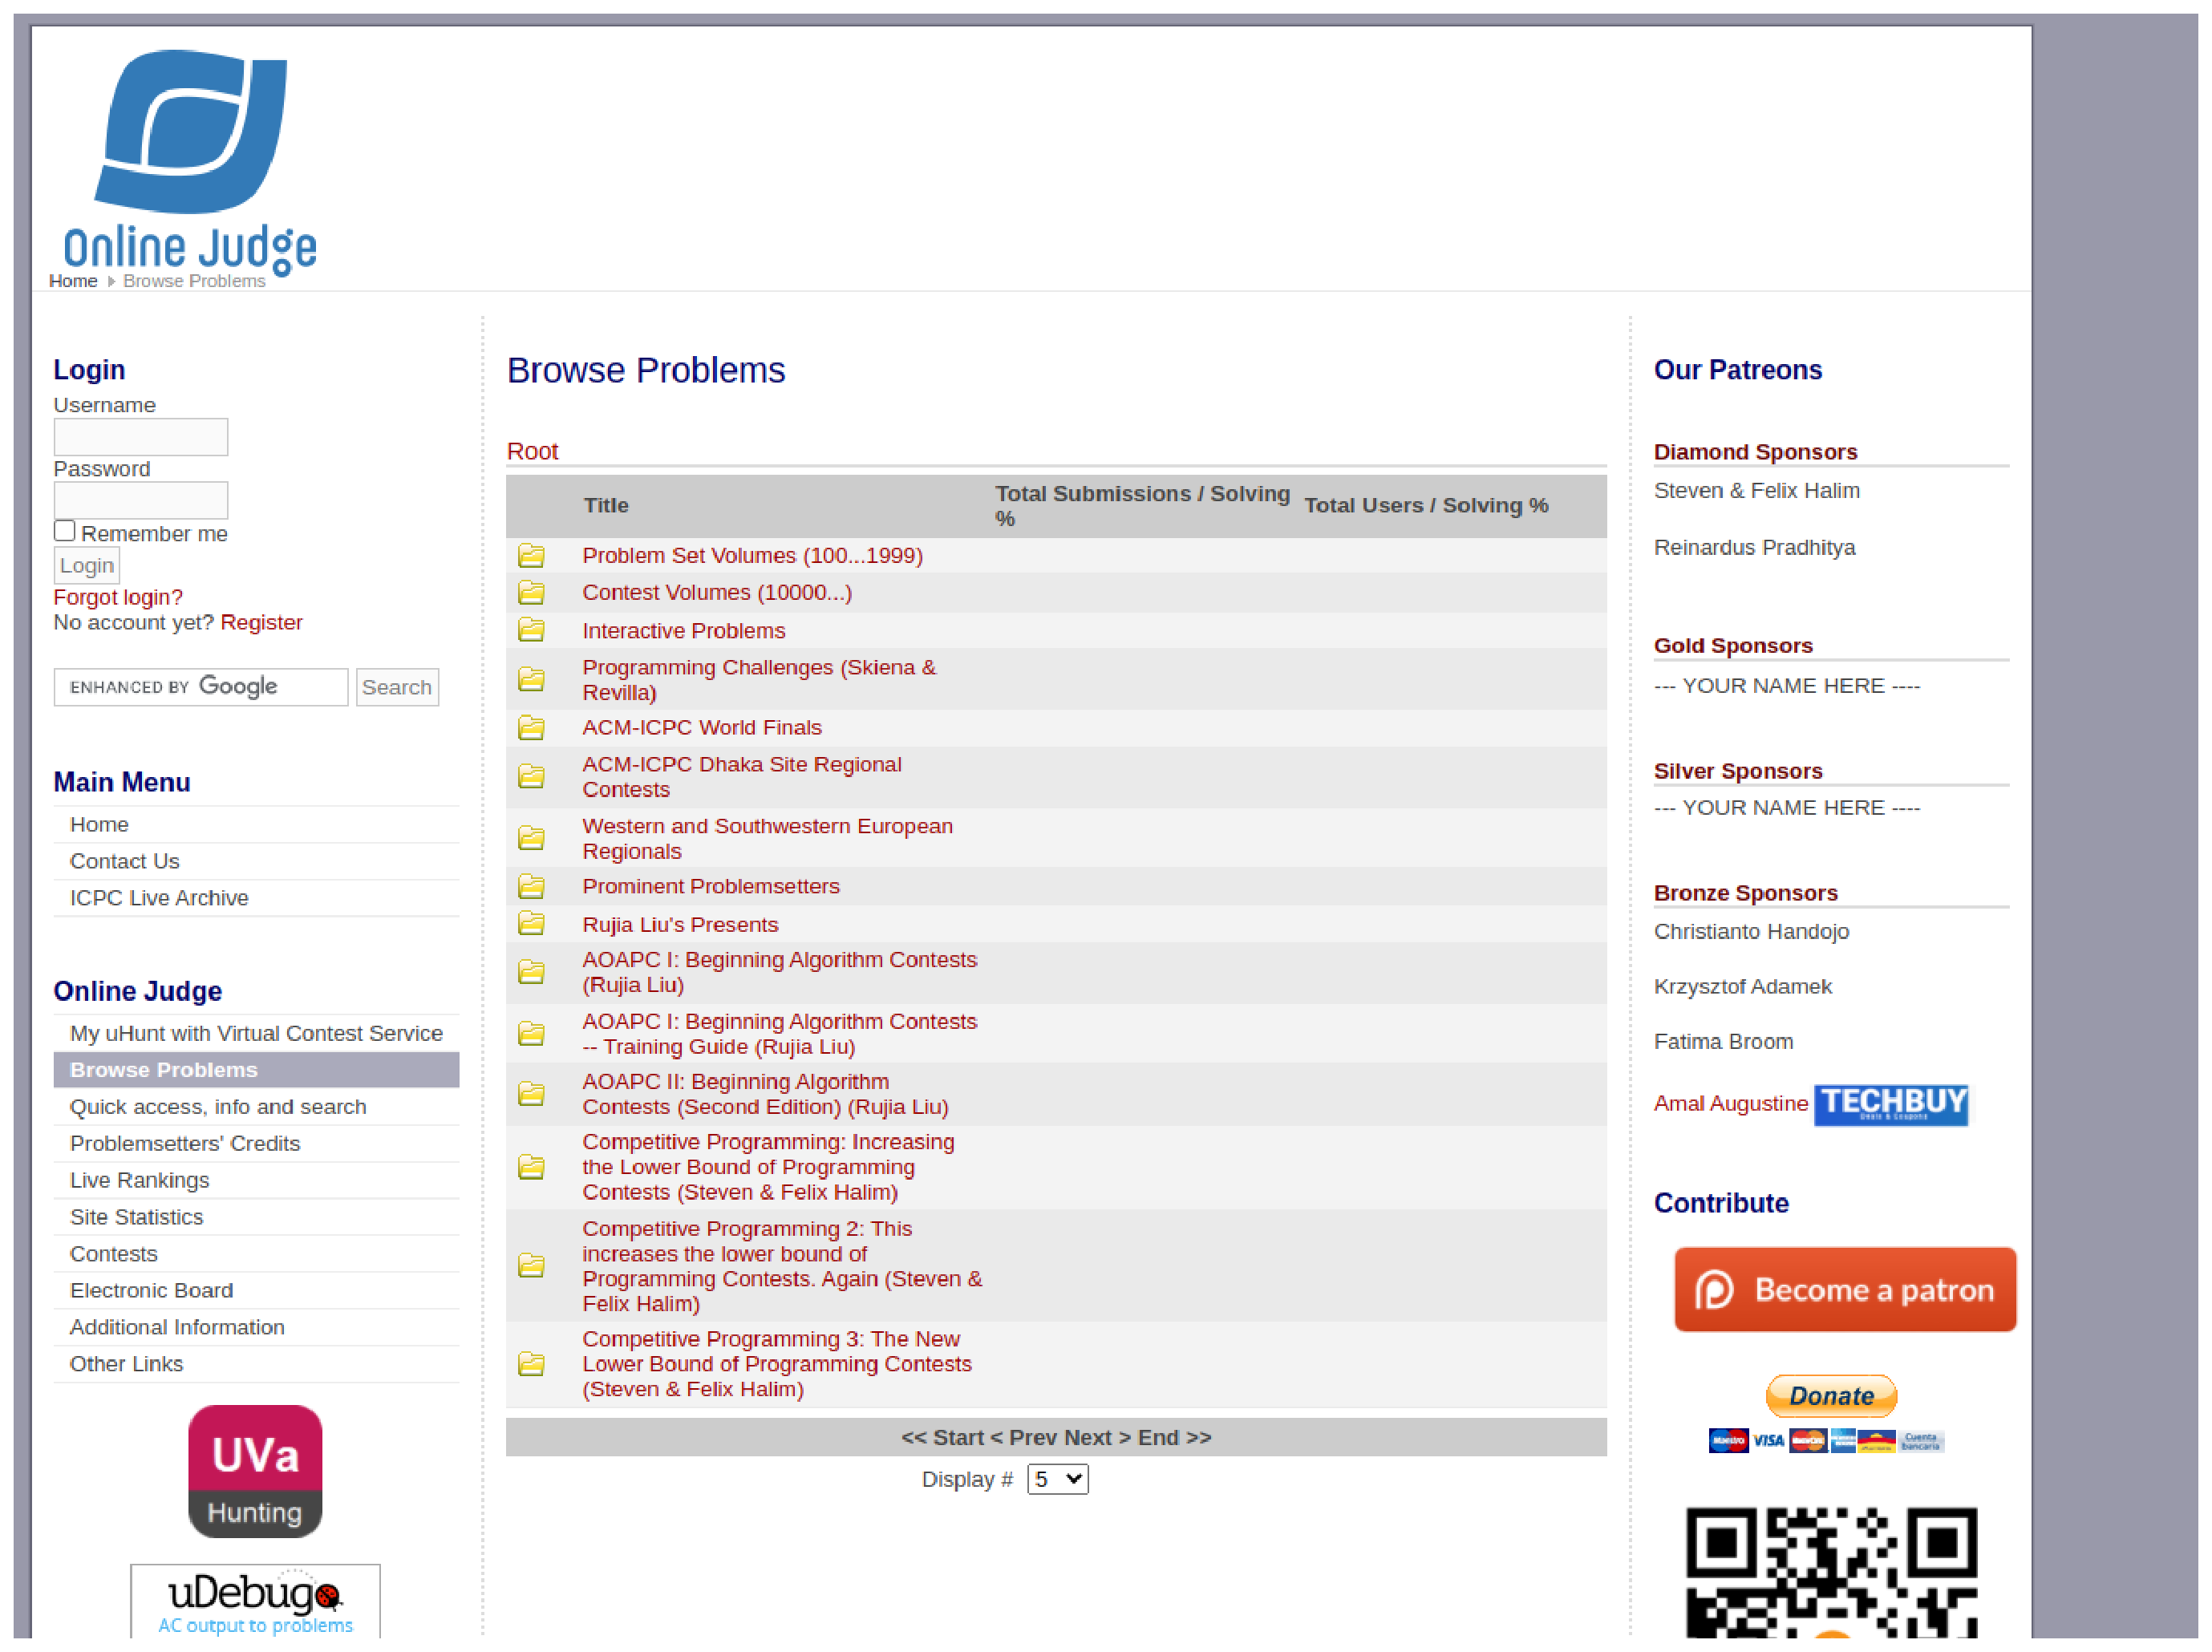
\includegraphics[keepaspectratio=true,scale=0.32]{figuras/online_judge_1.eps}
    \label{fig:online_judge_1}
\end{figure}

\begin{figure}[H]
    \centering
    \caption{Online Judge - Browse Problems (Detalhes)}
    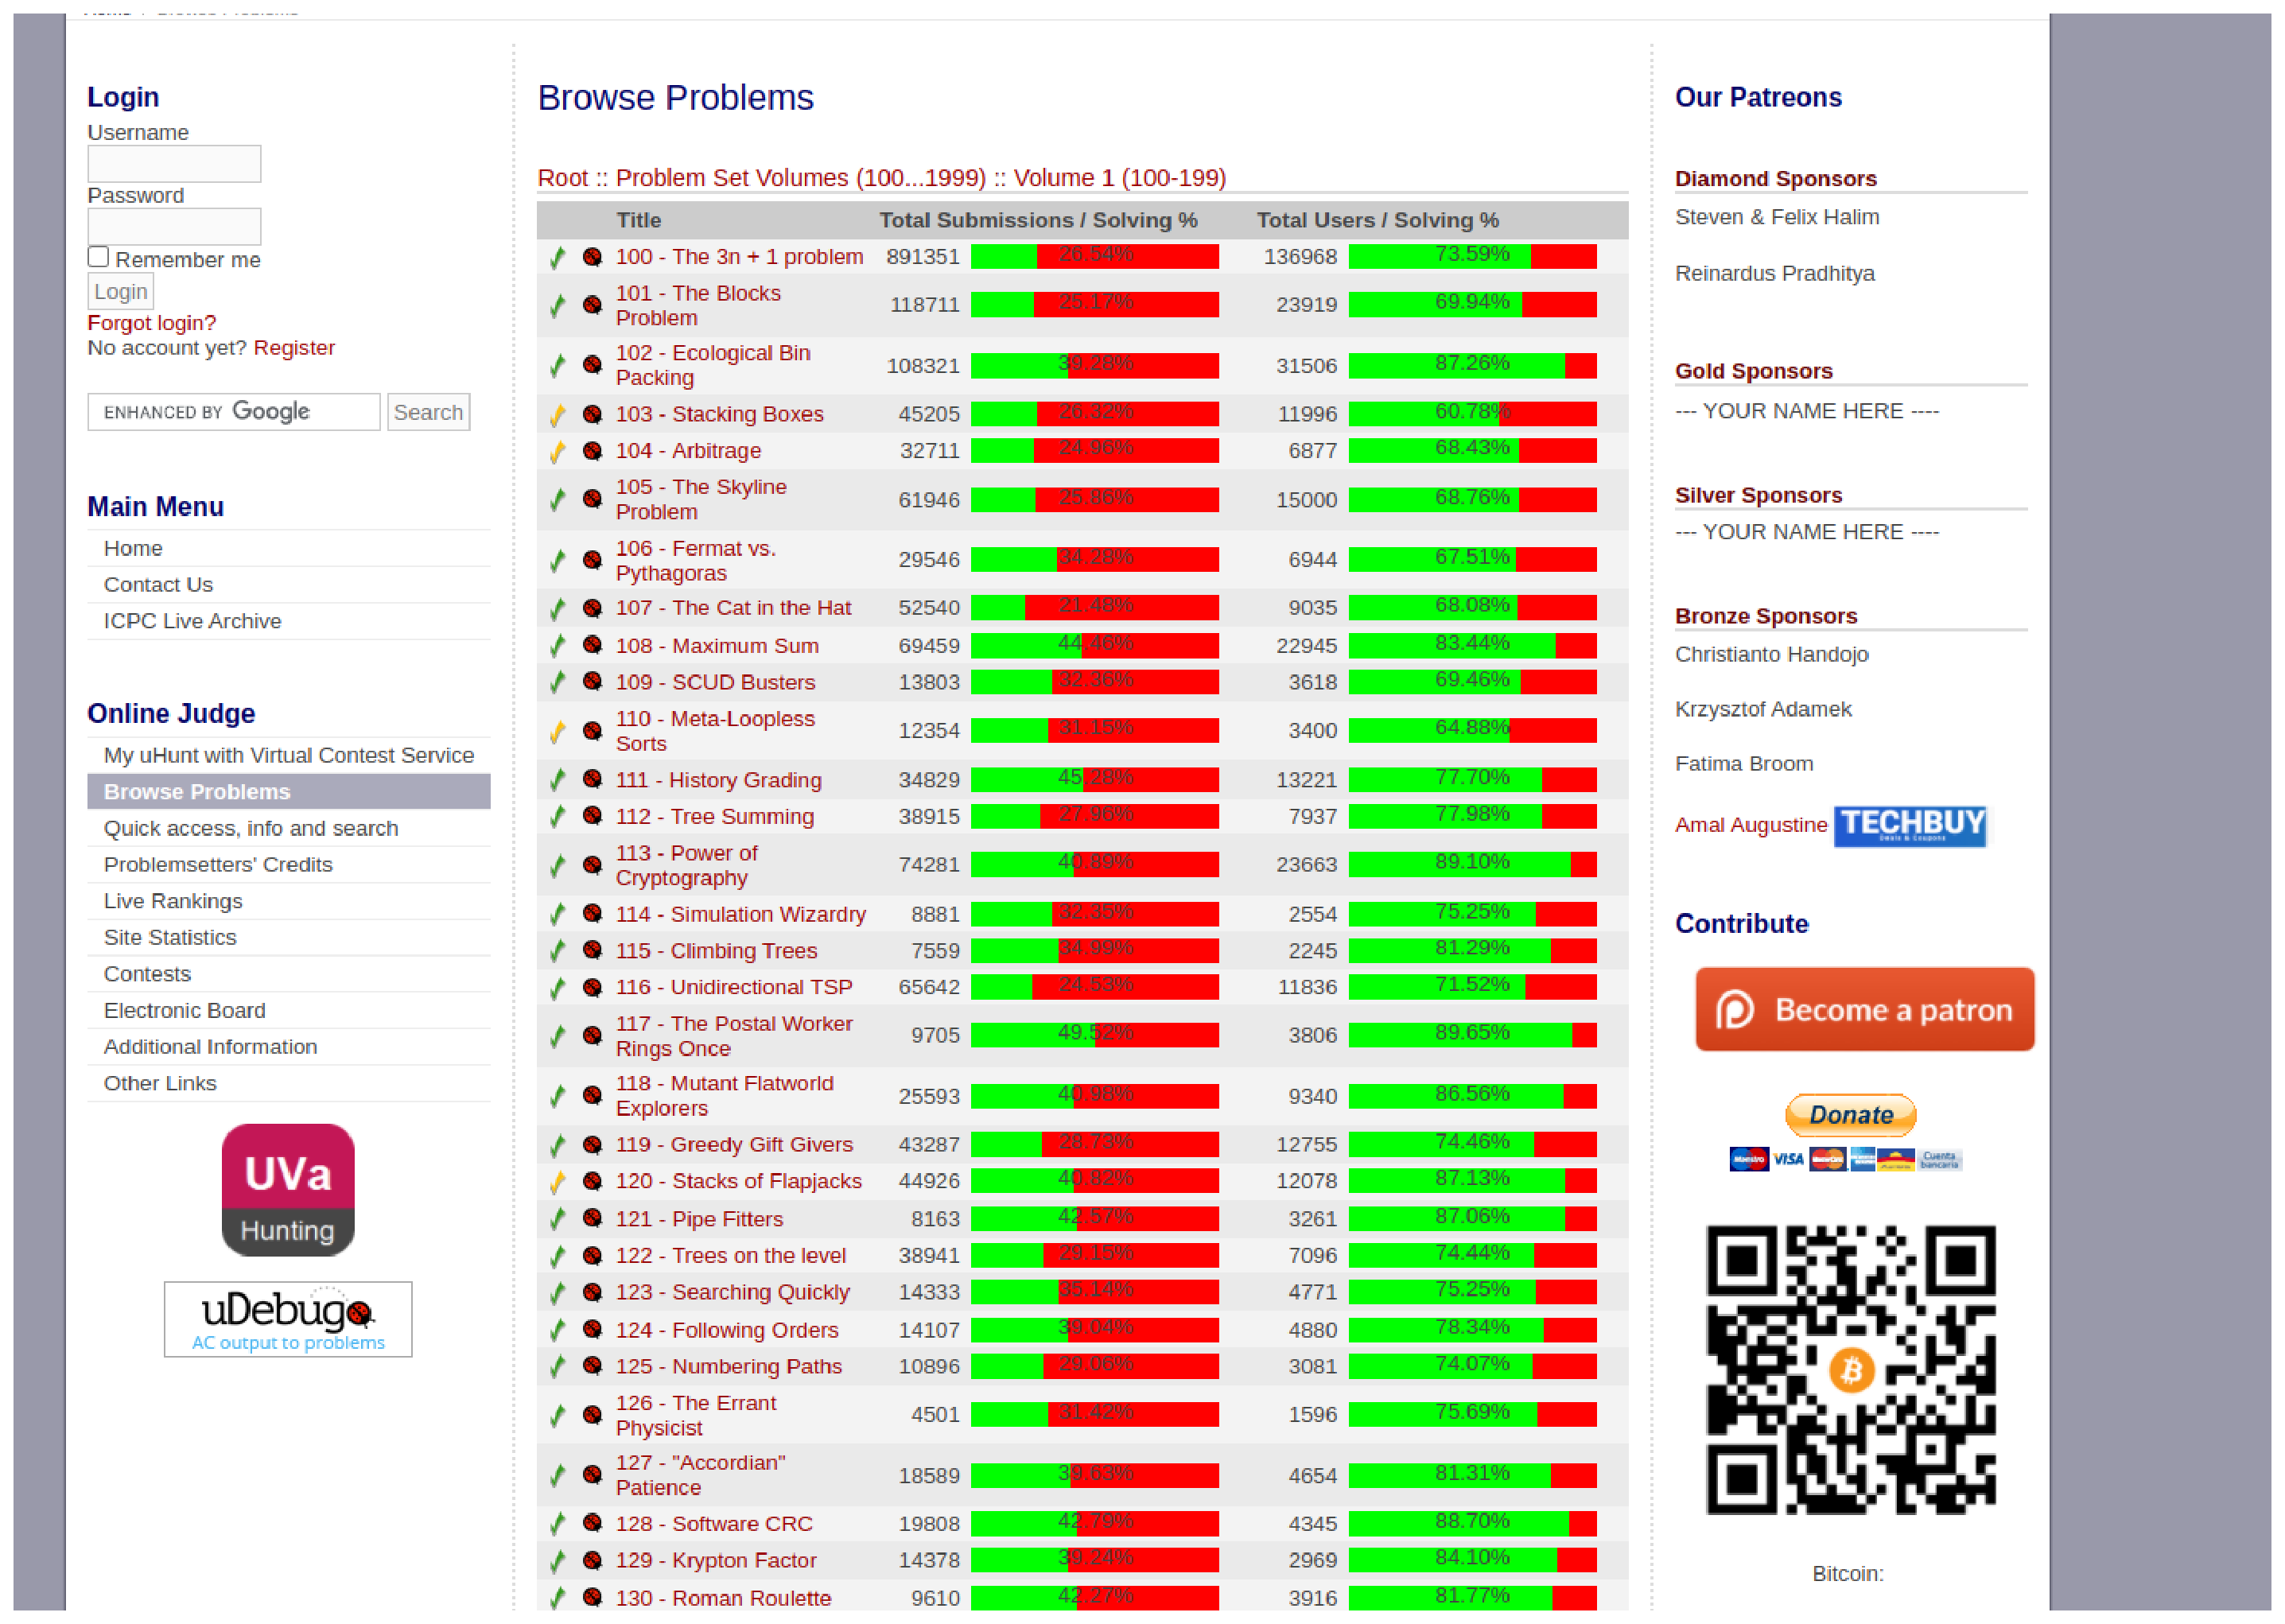
\includegraphics[keepaspectratio=true,scale=0.32]{figuras/online_judge_2.eps}
    \label{fig:online_judge_2}
\end{figure}

\begin{figure}[H]
    \centering
    \caption{Beecrowd - Total de problemas}
    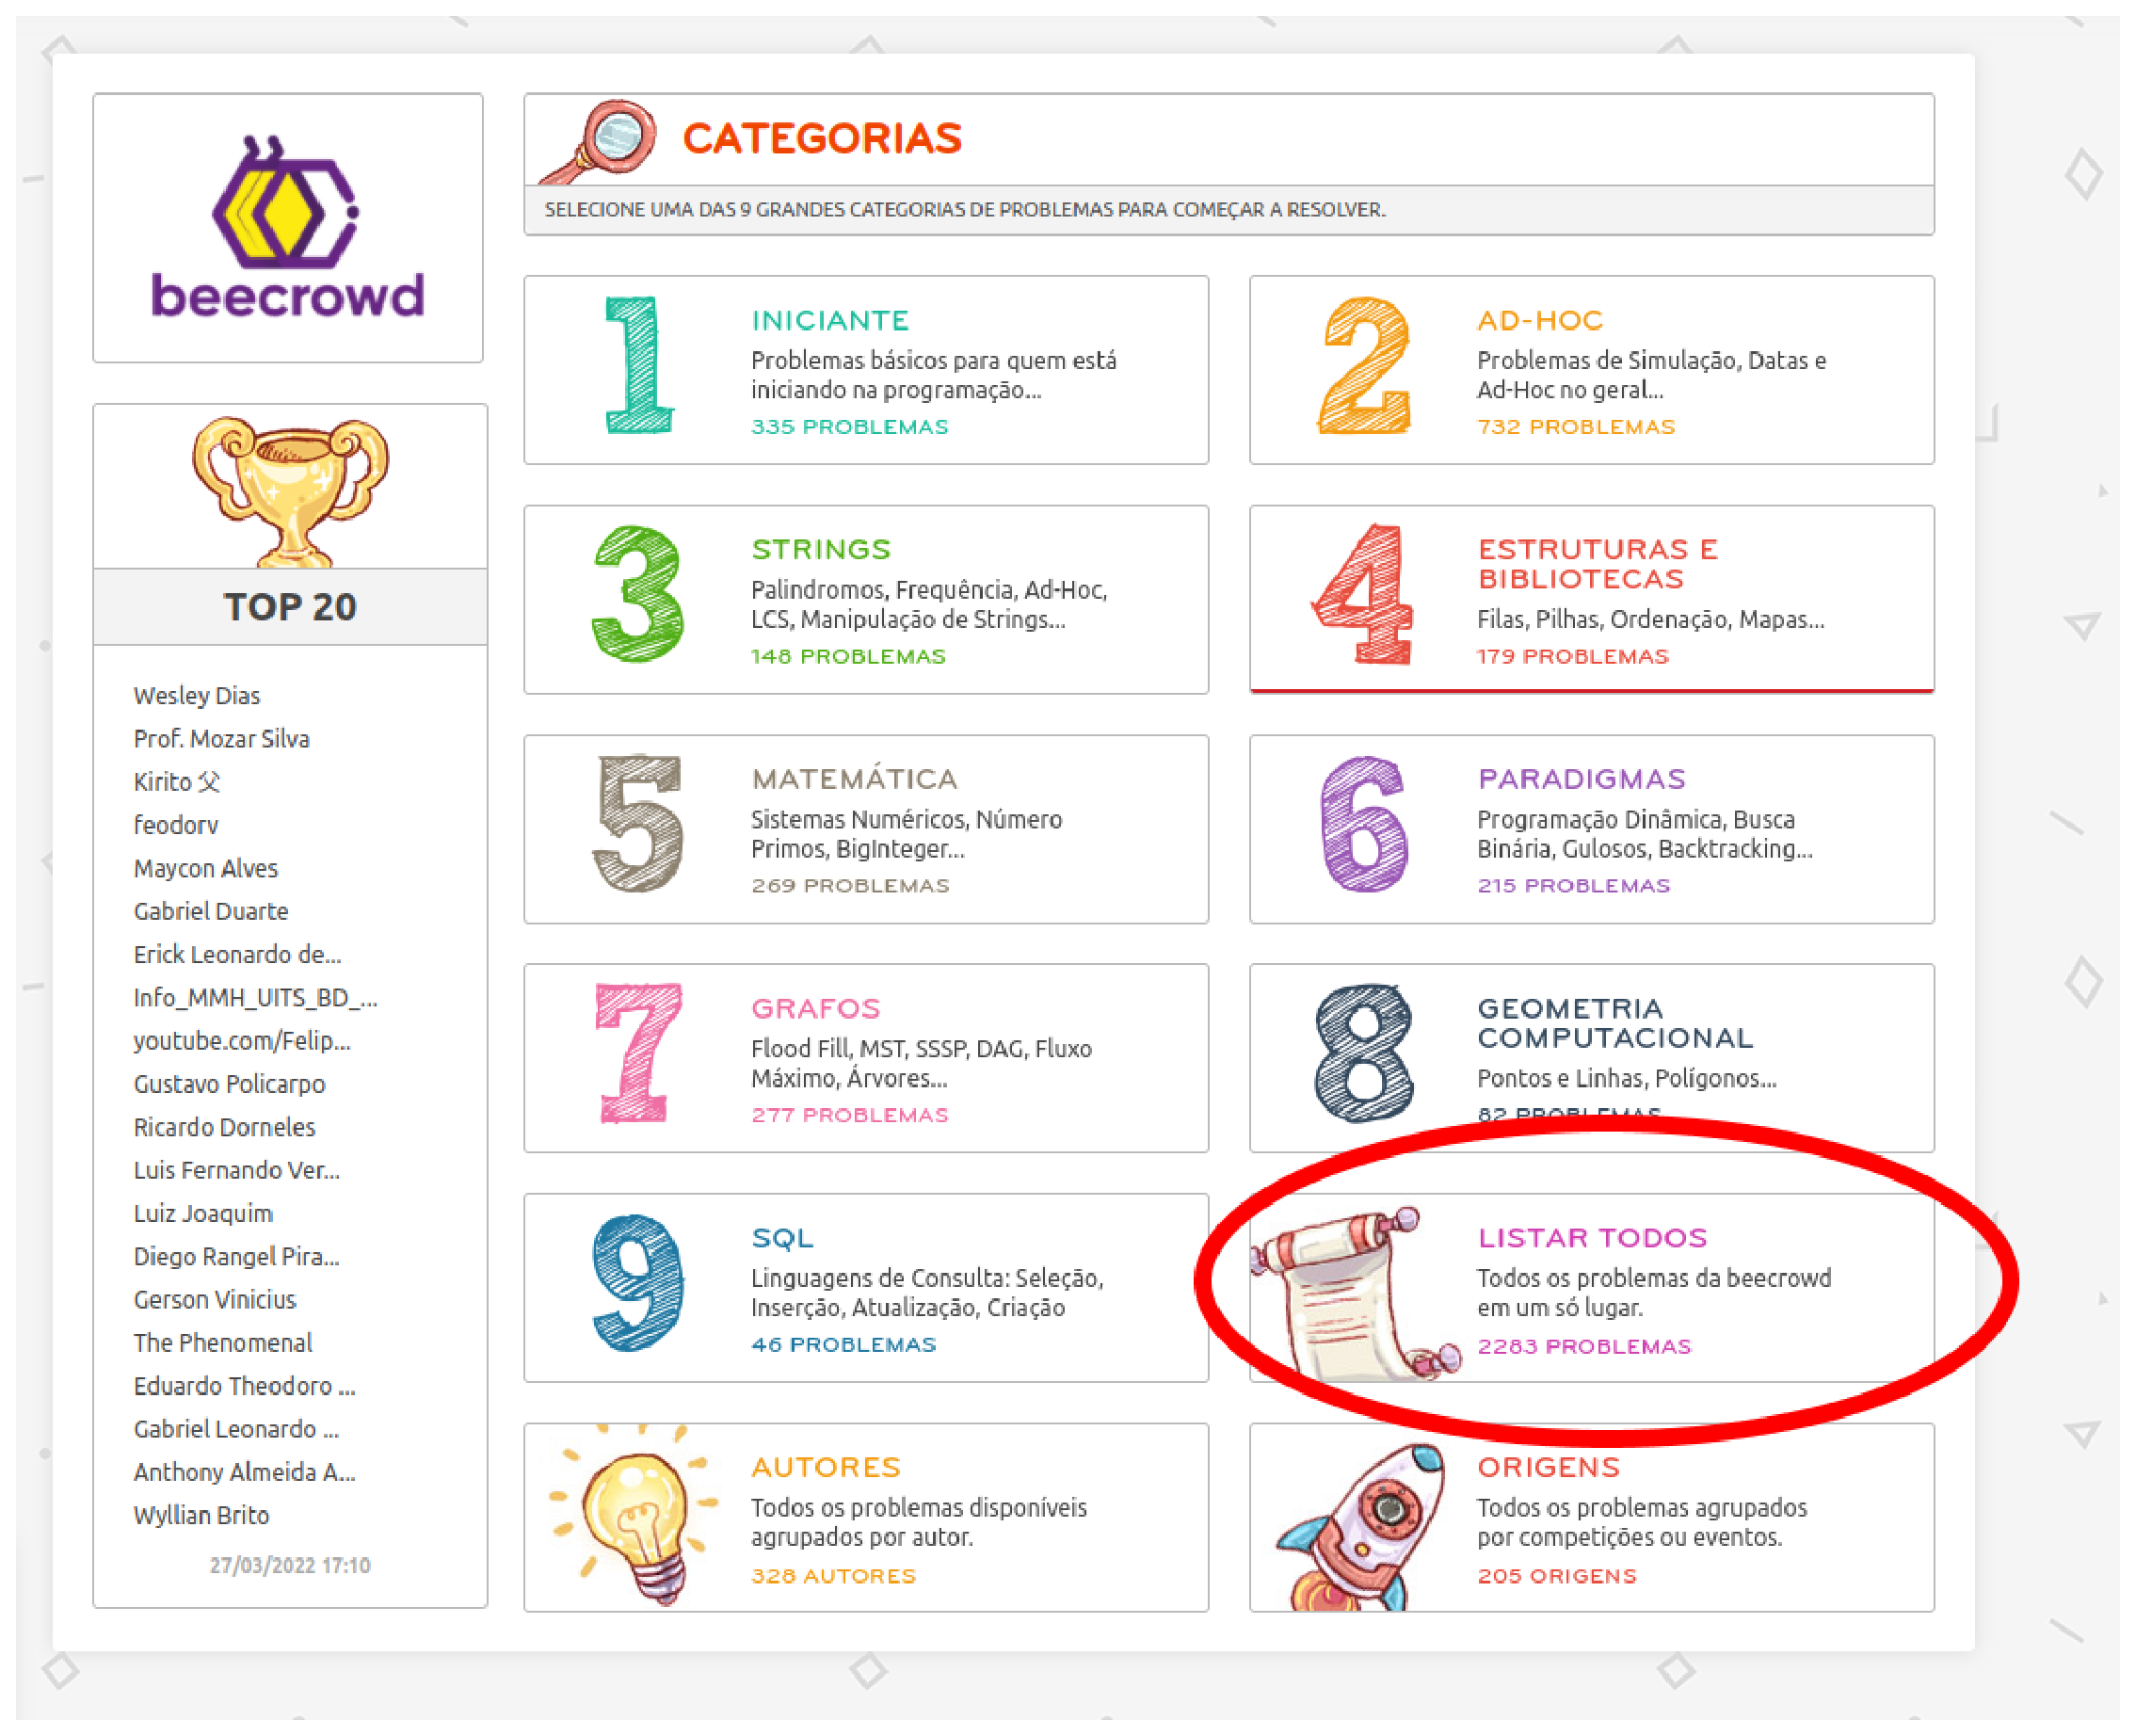
\includegraphics[keepaspectratio=true,scale=0.4]{figuras/beecrowd_1.eps}
    \label{fig:beecrowd_1}
\end{figure}

\begin{figure}[H]
    \centering
    \caption{Sphere Online Judge - Categorias de problemas}
    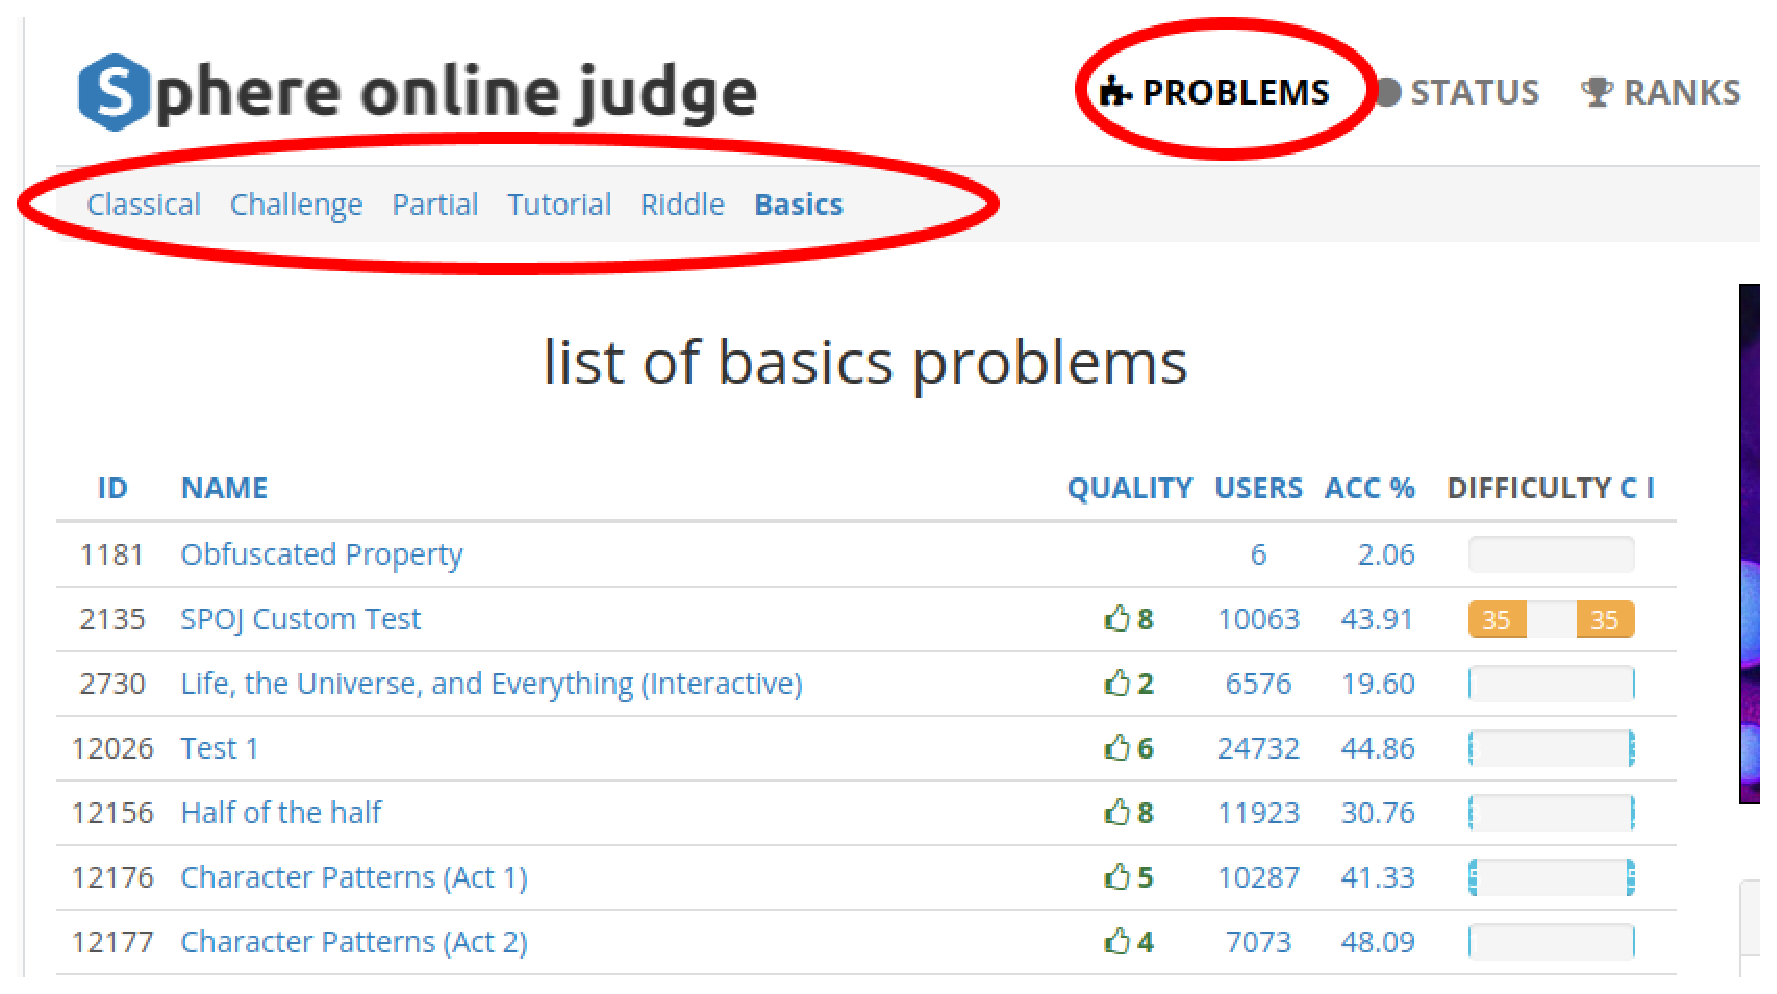
\includegraphics[keepaspectratio=true,scale=0.4]{figuras/spoj.eps}
    \label{fig:spoj}
\end{figure}


\begin{figure}[H]
    \centering
    \caption{PKU Judge Online - Problemas}
    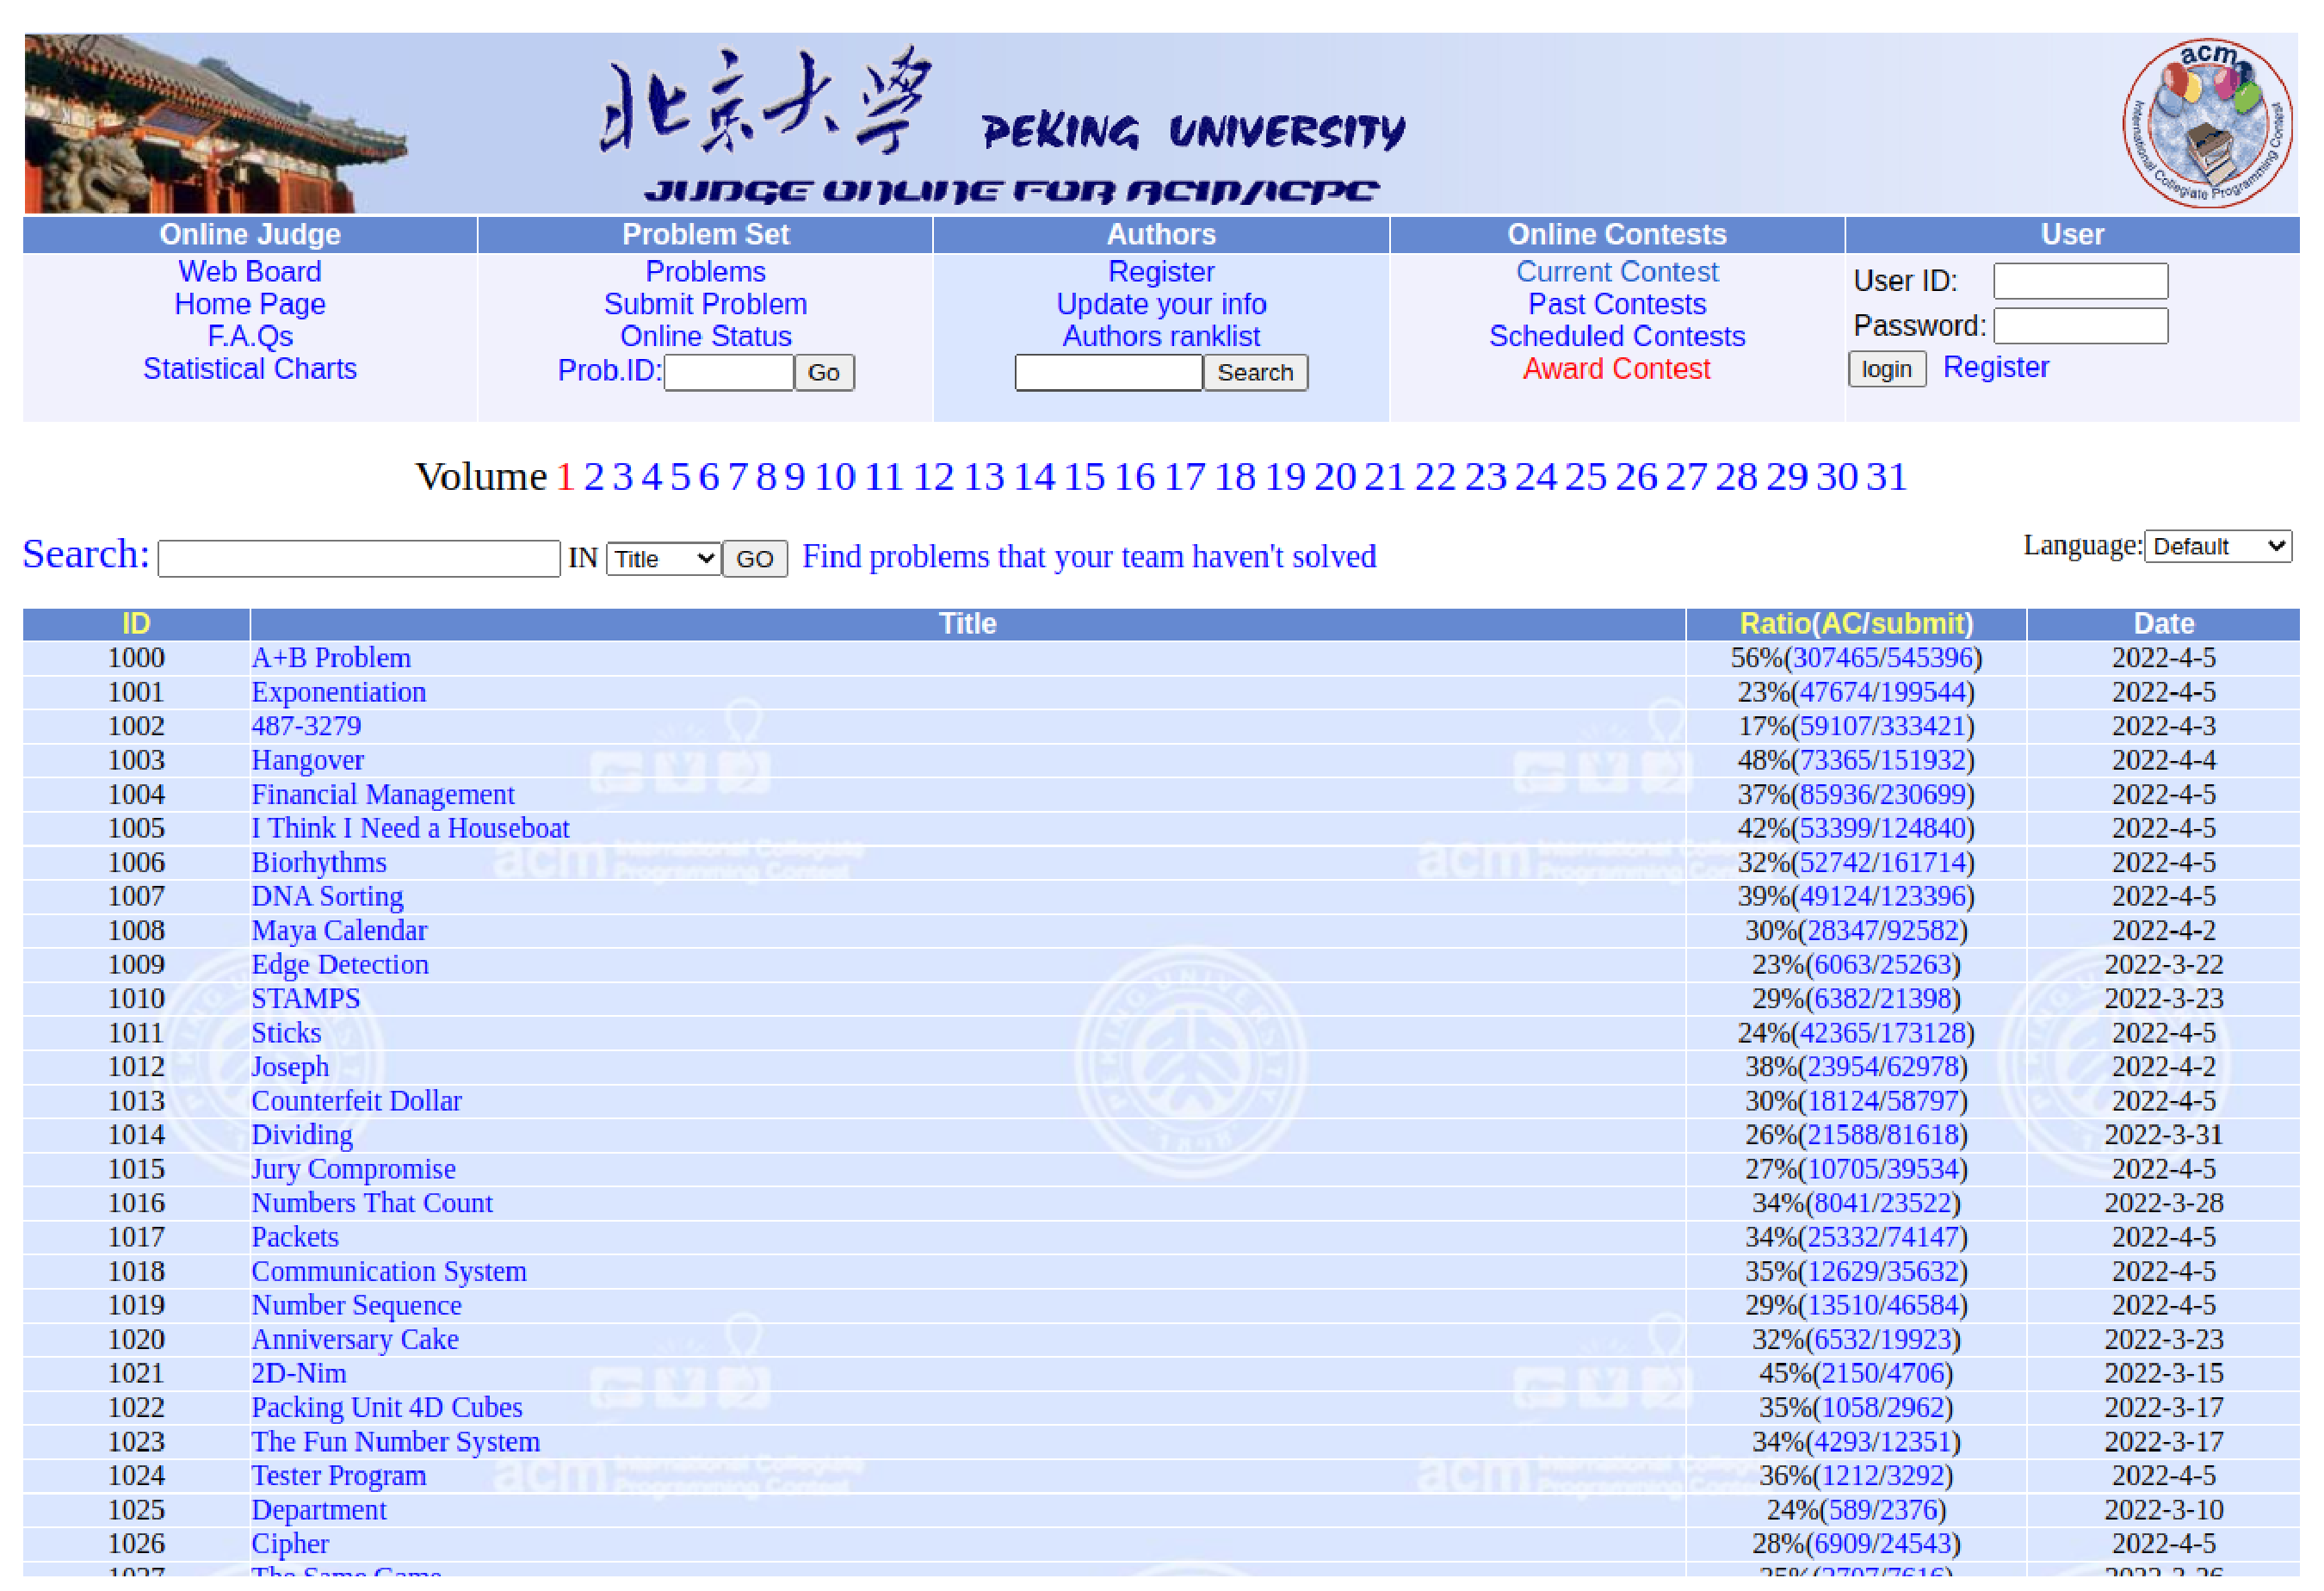
\includegraphics[keepaspectratio=true,scale=0.35]{figuras/pku.eps}
    \label{fig:pku}
\end{figure}

\begin{figure}[H]
    \centering
    \caption{PKU Judge Online - Compiladores}
    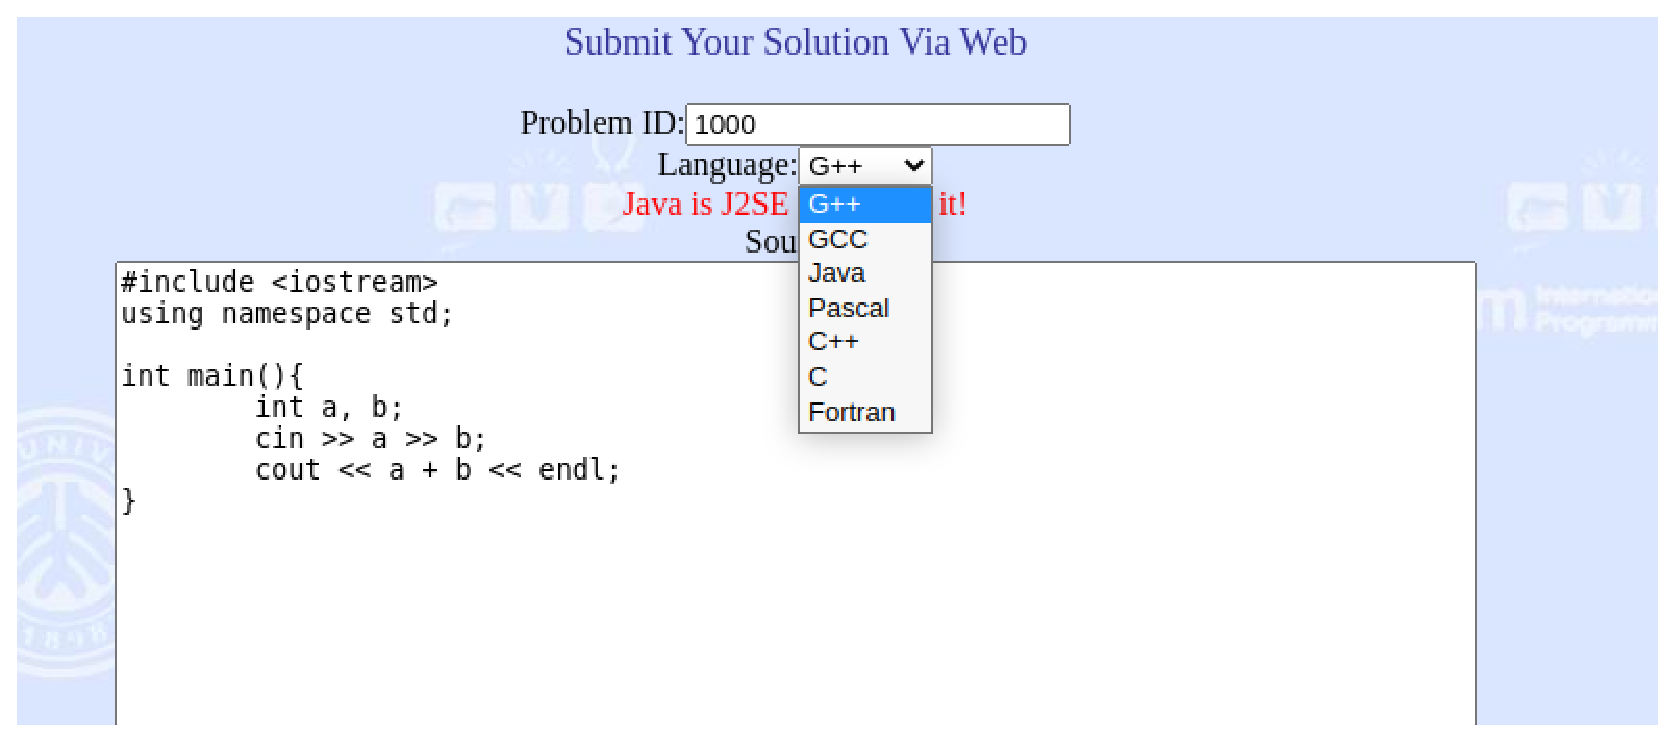
\includegraphics[keepaspectratio=true,scale=0.4]{figuras/pku_2.eps}
    \label{fig:pku_2}
\end{figure}

\begin{figure}[H]
    \centering
    \caption{Code Chef - Filtro de problemas}
    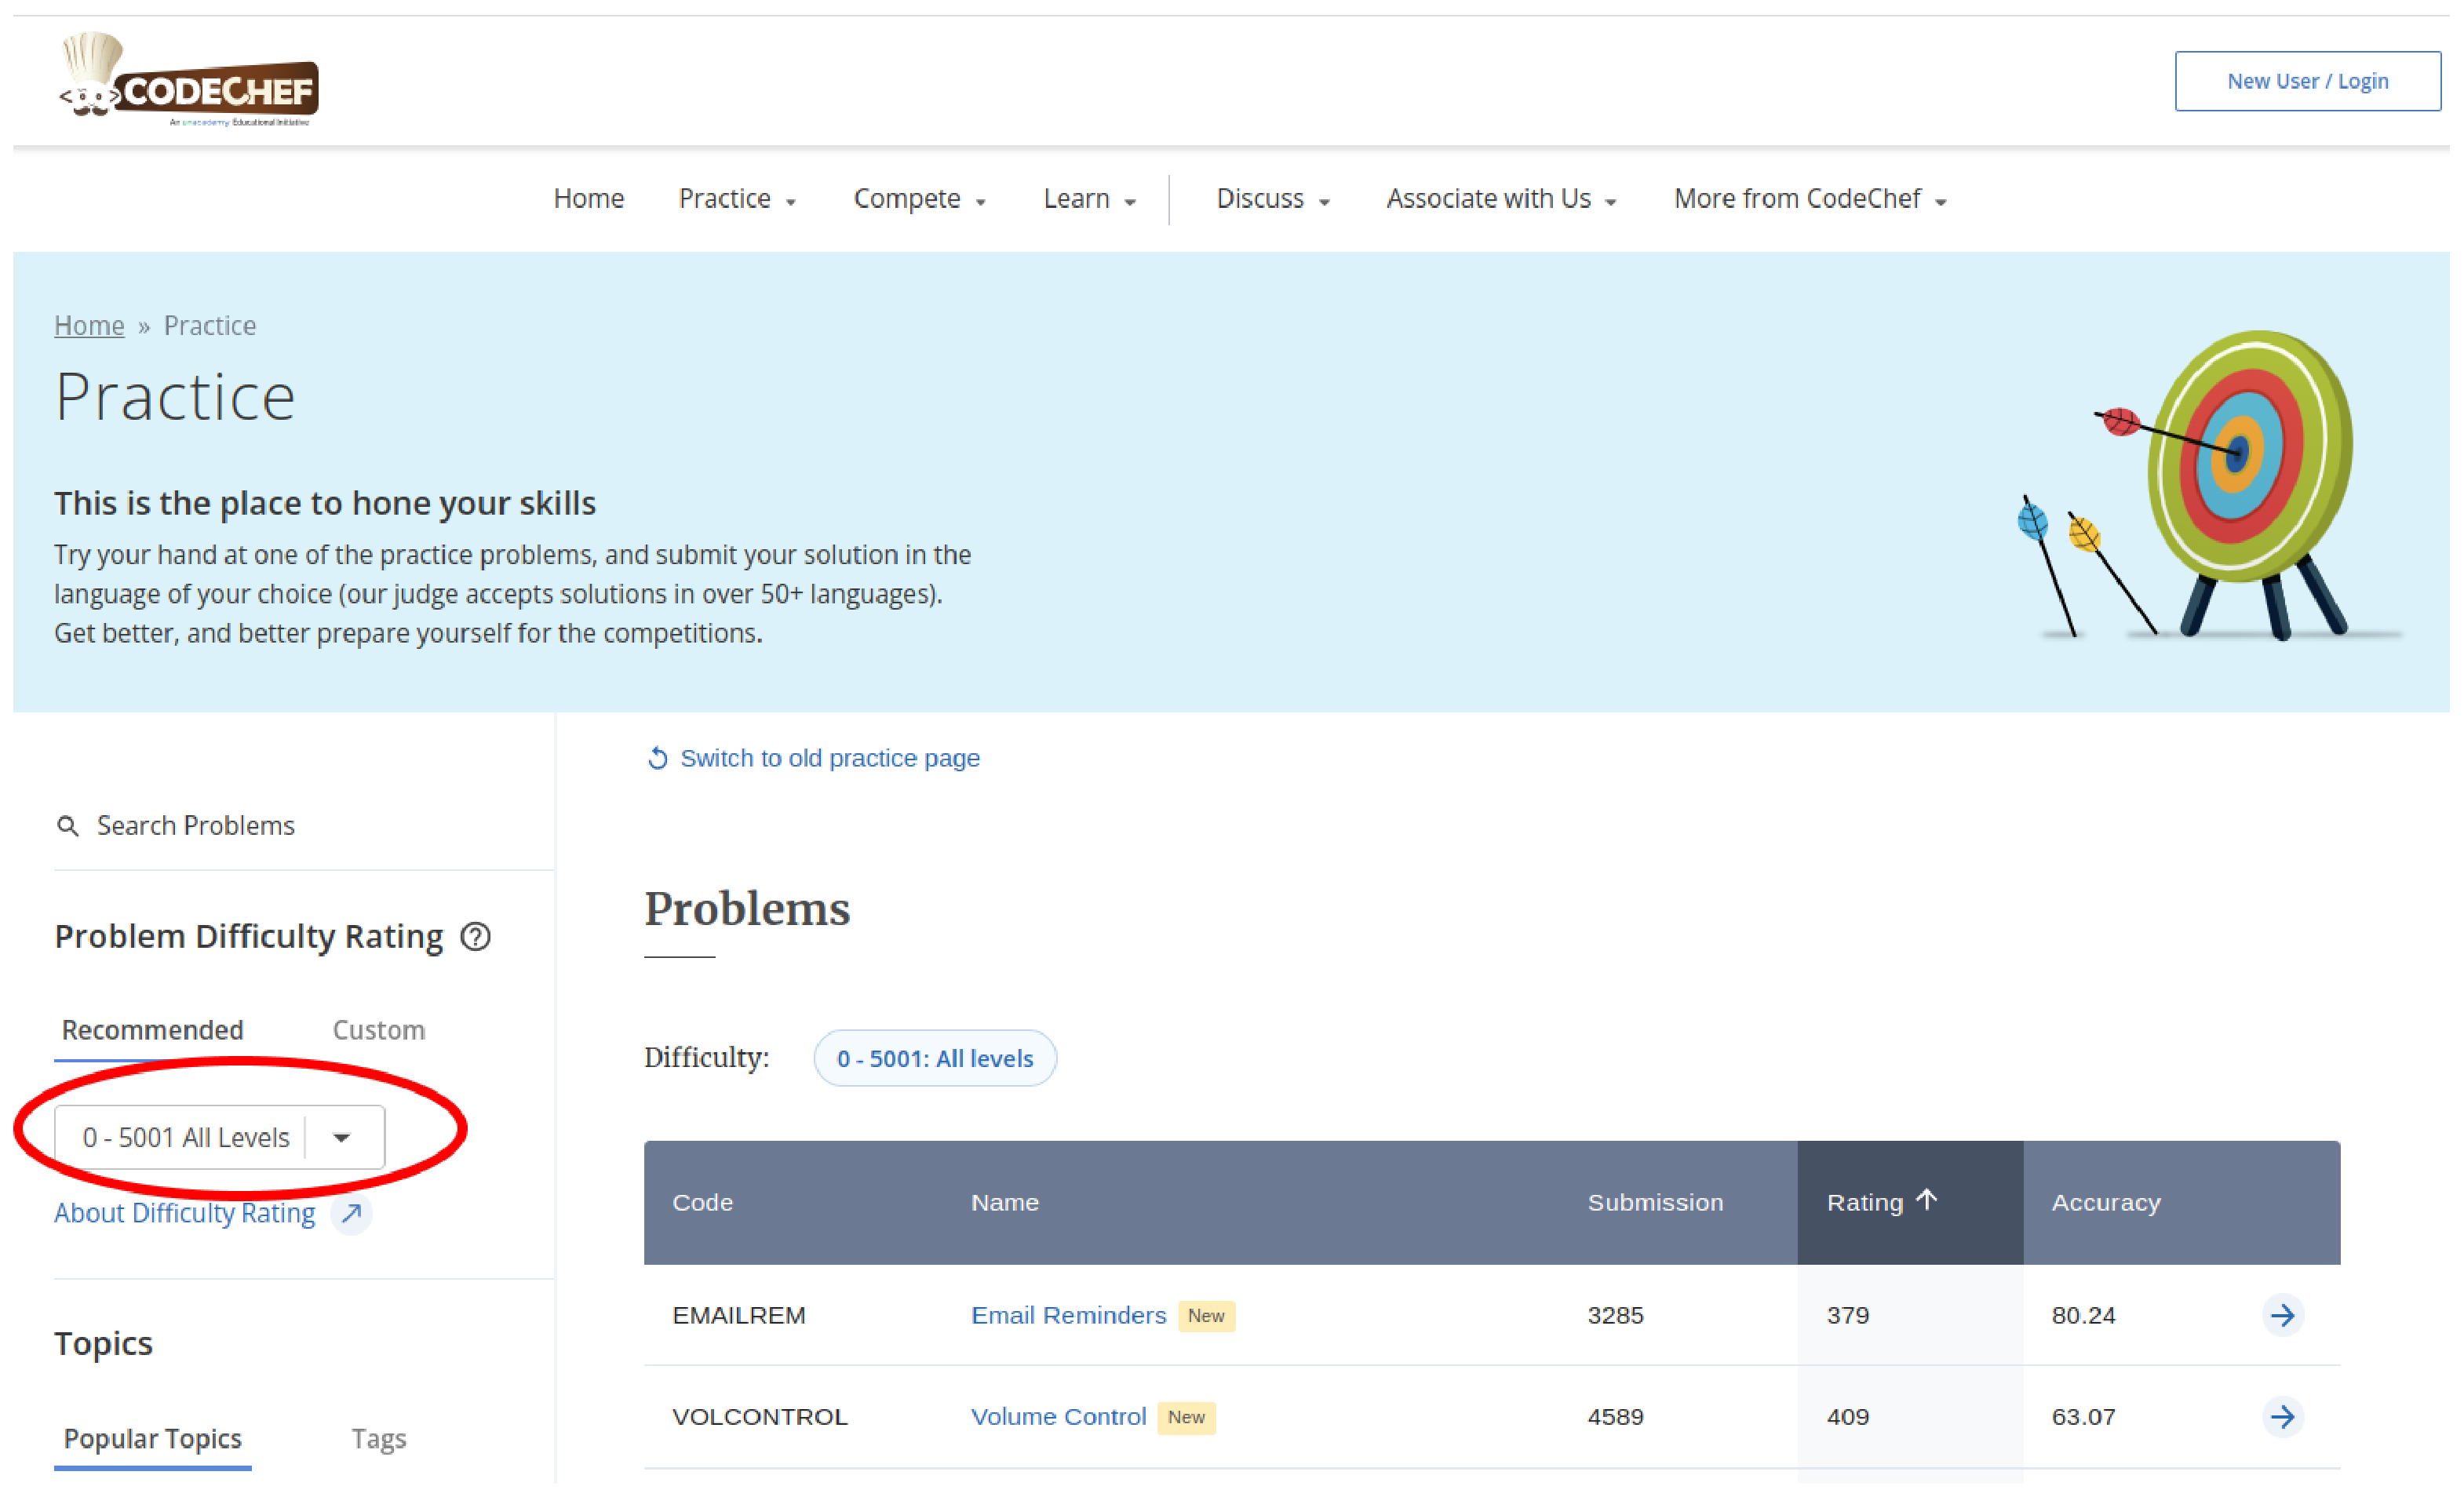
\includegraphics[keepaspectratio=true,scale=0.3]{figuras/code_chef_1.eps}
    \label{fig:code_chef_1}
\end{figure}

\begin{figure}[H]
    \centering
    \caption{Code Chef - Número de problemas}
    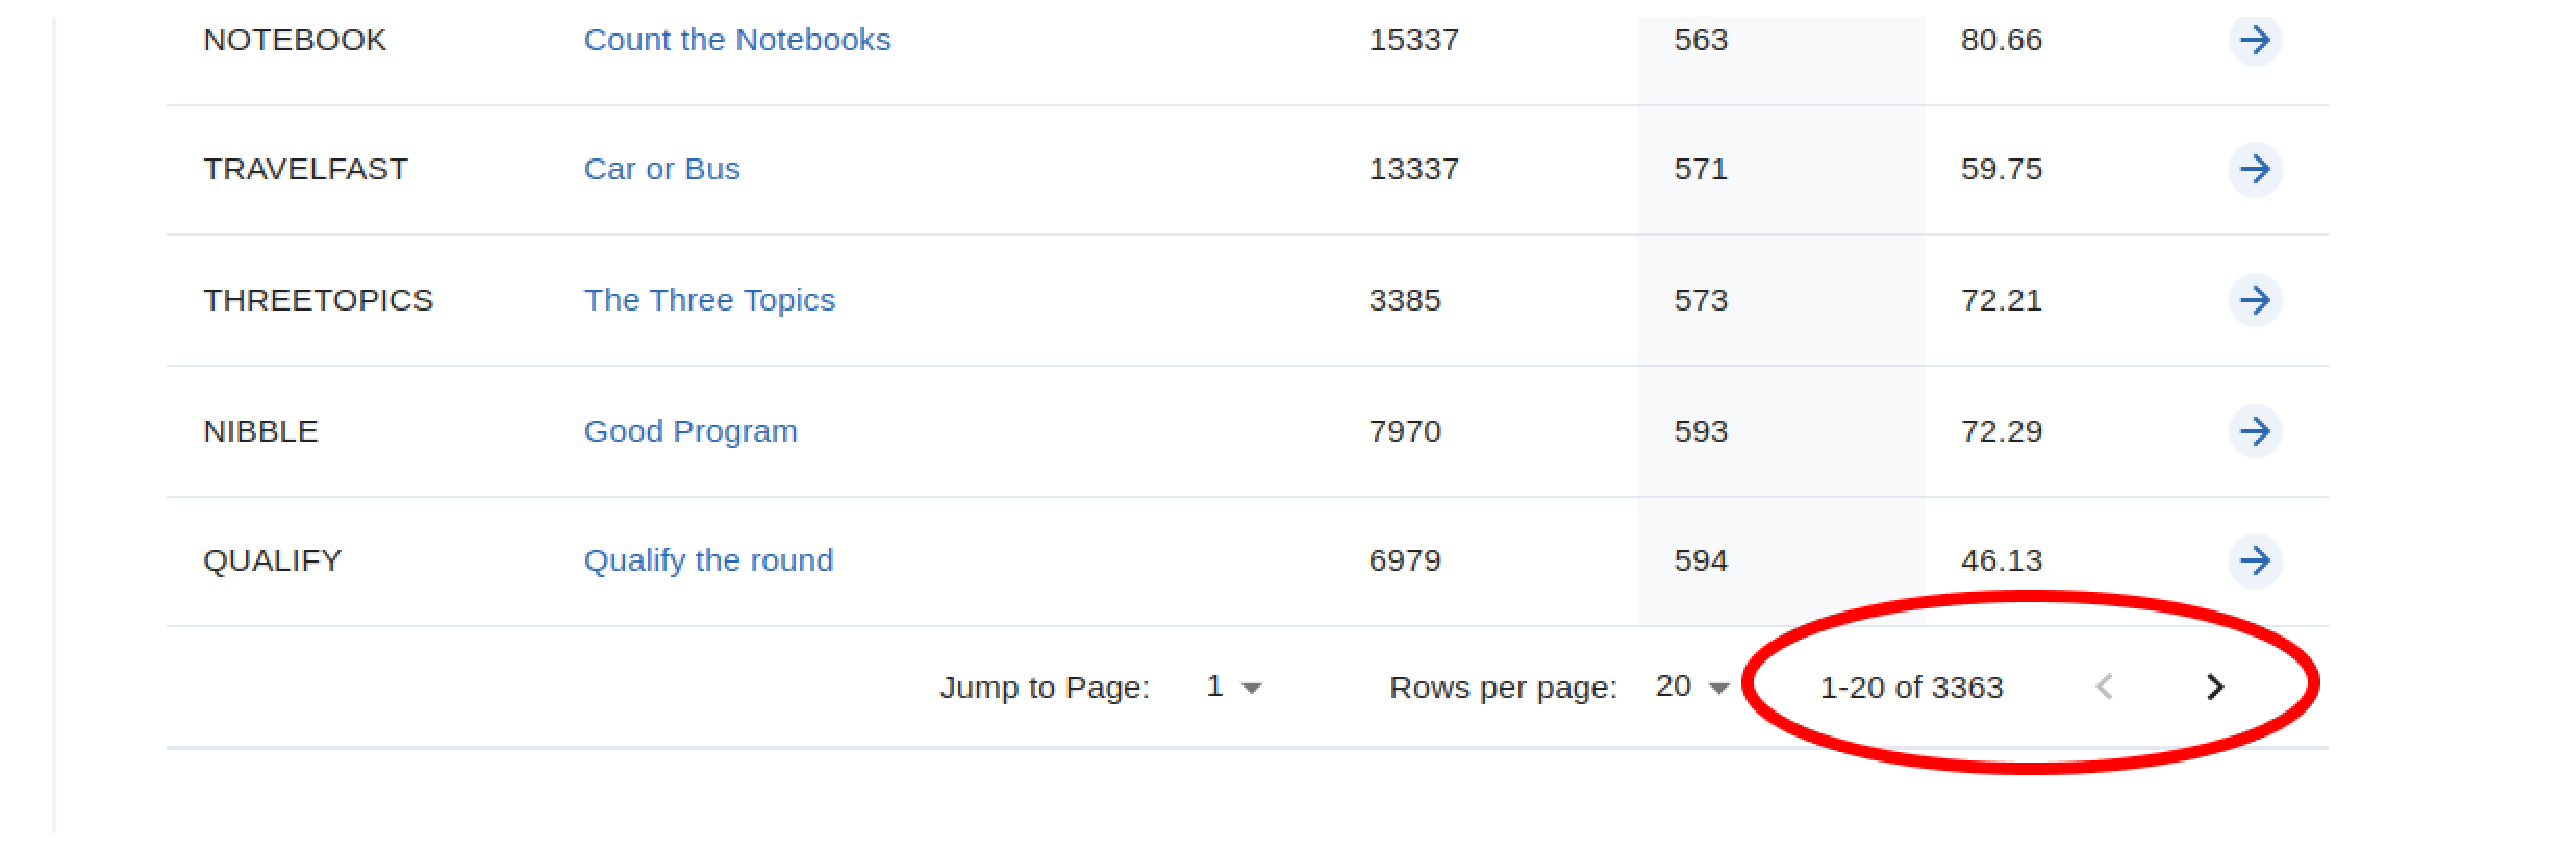
\includegraphics[keepaspectratio=true,scale=0.3]{figuras/code_chef_2.eps}
    \label{fig:code_chef_2}
\end{figure}

\chapter{Segundo Anexo}

    Texto do segundo anexo.

\end{anexosenv}

